\documentclass[11pt,a4paper]{article}

\usepackage[utf8]{inputenc}
\usepackage[margin=1in]{geometry}
\usepackage{amsmath,amssymb}
\usepackage{booktabs}
\usepackage{tabularx}
\usepackage{hyperref}
\usepackage{listings}
\usepackage{xcolor}
\usepackage{fancyhdr}
\usepackage{enumitem}
\usepackage{microtype}
\usepackage{titlesec}
\usepackage{tikz}
\usetikzlibrary{shapes.geometric, arrows, positioning}

% Hyperlink configuration
\hypersetup{
    colorlinks=true,
    linkcolor=blue!70!black,
    citecolor=blue!70!black,
    urlcolor=blue!70!black
}

% Code listing configuration
\definecolor{codegreen}{rgb}{0,0.6,0}
\definecolor{codegray}{rgb}{0.5,0.5,0.5}
\definecolor{codepurple}{rgb}{0.58,0,0.82}
\definecolor{backcolour}{rgb}{0.96,0.96,0.96}

\lstdefinestyle{mystyle}{
    backgroundcolor=\color{backcolour},   
    commentstyle=\color{codegreen},
    keywordstyle=\color{magenta},
    numberstyle=\tiny\color{codegray},
    stringstyle=\color{codepurple},
    basicstyle=\ttfamily\footnotesize,
    breakatwhitespace=false,         
    breaklines=true,                 
    captionpos=b,                    
    keepspaces=true,                 
    numbers=left,                    
    numbersep=5pt,                  
    showspaces=false,                
    showstringspaces=false,
    showtabs=false,                  
    tabsize=2
}
\lstset{style=mystyle}

% Header and Footer
\pagestyle{fancy}
\fancyhf{}
\rhead{\footnotesize Confluentia 2026 --- Reliable Video Transfer \& Frame Integrity Analysis}
\lhead{\footnotesize Technical Challenge Report}
\rfoot{\thepage}

\title{\textbf{\Large Fault-Tolerant Video Transfer Protocol and 30 FPS Frame-Level Integrity Analysis Service}\\[0.4em]
\large Confluentia 2026 Technical Challenge Submission\\
\normalsize Organizers: IIT BHU, Nihilent / nSEPIA}
\author{\textbf{Candidate Submission} \\
GitHub: \href{https://github.com/SIDDHARTH2751/PROJECTS}{SIDDHARTH2751/PROJECTS}}
\date{November 15, 2026}

\begin{document}

\maketitle

\begin{abstract}
Transmitting video assets reliably over unpredictable and hostile wireless networks while guaranteeing both transport-level and media-level integrity is a critical requirement in autonomous systems, surveillance, and edge media processing. This paper presents an end-to-end engineered solution for the Confluentia 2026 Technical Challenge. The system comprises: (1) a chunked, resumable, and cryptographically verified HTTP/REST video transfer protocol; (2) a configurable software-defined TCP fault proxy capable of dynamically simulating variable bandwidth (20\%--100\%), latency jitter, connection resets, hung sockets, blackouts, and payload corruption; and (3) a hard-gated 30 FPS frame-level video integrity analyzer built on FFmpeg, PyAV, and OpenCV. We detail the protocol state machine, atomic storage mechanics, randomized backoff algorithm, multi-vector anomaly detection (PTS gaps, freeze runs, VFR drift), and deterministic root-cause classification logic. Comprehensive validation across 20 automated unit tests and 10 end-to-end degraded network scenarios demonstrates zero-loss transfer resilience and sub-frame forensic diagnostic accuracy.
\end{abstract}

\vspace{0.5em}
\noindent\textbf{Keywords:} Resumable Video Ingestion, Cryptographic Verification, Network Fault Injection, Frame-Level Forensic Analysis, PTS Discontinuity, Confluentia 2026.

\section{Introduction and Problem Formulation}

Modern video ingestion pipelines regularly interface with unstable cellular or edge environments characterized by bandwidth throttling, transient link drops, packet loss, and latency variance. For mission-critical media streams (such as 30-second surveillance or diagnostic recordings at 30 FPS), system failures manifest in two distinct domains:
\begin{enumerate}[leftmargin=*,itemsep=1pt]
    \item \textbf{Transport Insecurity}: Data streams truncated, packets corrupted in transit, or upload sessions aborted midway due to network disconnects.
    \item \textbf{Media Integrity Violations}: Video streams with missing frames, presentation timestamp (PTS) discontinuities, frozen frame sequences, or variable frame rate (VFR) drift caused by upstream camera sensor throttling or encoding underruns.
\end{enumerate}

The challenge requires engineering a client-server architecture capable of delivering a 30-second video over simulated 20\%--100\% signal fluctuations, followed by automated forensic analysis. Crucially, the system must establish the fundamental technical distinction: \emph{a byte-perfect transfer cannot prove that the original recording was free of dropped frames}. This report documents the architecture, formal protocols, anomaly algorithms, and empirical verification of the completed implementation.

\section{System Architecture and Transfer Protocol}

\subsection{Architectural Topology}
The solution is organized into three decoupled subsystems: the Client Uploader, the Fault-Injecting Proxy, and the FastAPI Backend with its Hard-Gated Analytical Engine.

\begin{figure}[htbp]
\centering
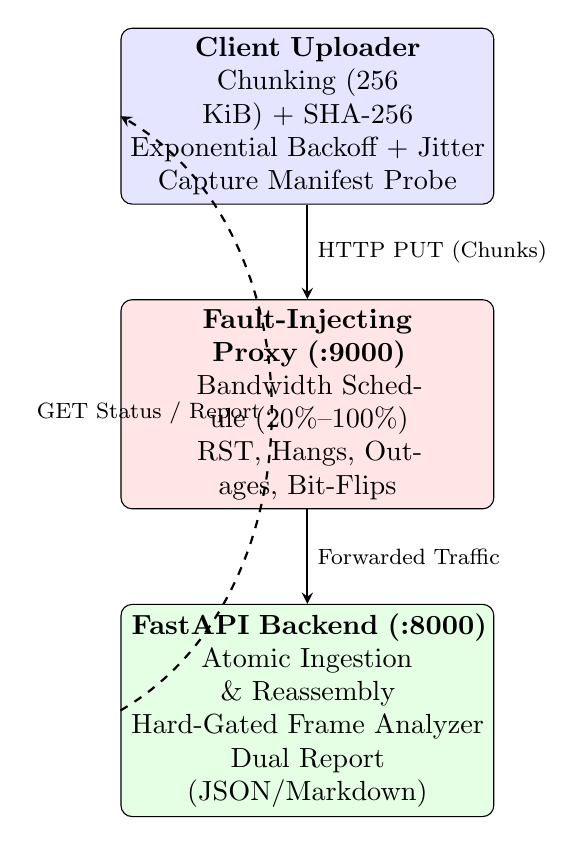
\begin{tikzpicture}[node distance=1.2cm, auto,
    block/.style={rectangle, draw, fill=blue!10, text width=4.5cm, text centered, rounded corners, minimum height=1cm},
    proxy/.style={rectangle, draw, fill=red!10, text width=4.5cm, text centered, rounded corners, minimum height=1cm},
    server/.style={rectangle, draw, fill=green!10, text width=4.5cm, text centered, rounded corners, minimum height=1cm},
    arrow/.style={thick,->,>=stealth}]
    
    \node [block] (client) {\textbf{Client Uploader}\\Chunking (256 KiB) + SHA-256\\Exponential Backoff + Jitter\\Capture Manifest Probe};
    \node [proxy, below=of client] (proxy) {\textbf{Fault-Injecting Proxy (:9000)}\\Bandwidth Schedule (20\%--100\%)\\RST, Hangs, Outages, Bit-Flips};
    \node [server, below=of proxy] (server) {\textbf{FastAPI Backend (:8000)}\\Atomic Ingestion \& Reassembly\\Hard-Gated Frame Analyzer\\Dual Report (JSON/Markdown)};
    
    \draw [arrow] (client) -- node[right]{\footnotesize HTTP PUT (Chunks)} (proxy);
    \draw [arrow] (proxy) -- node[right]{\footnotesize Forwarded Traffic} (server);
    \draw [arrow, dashed] (server.west) to [bend right=60] node[left]{\footnotesize GET Status / Report} (client.west);
\end{tikzpicture}
\caption{End-to-End System Architecture and Communication Topology.}
\label{fig:arch}
\end{figure}

\subsection{State Machine Formalization}
The server guarantees crash consistency and data integrity through an explicit finite state machine (FSM). Session states are stored in a persistent JSON document alongside the chunk store:
\[
S \in \{\text{CREATED}, \text{UPLOADING}, \text{ASSEMBLED}, \text{VERIFIED}, \text{ANALYZED}, \text{FAILED}, \text{INCOMPLETE}\}
\]

\begin{itemize}[leftmargin=*,itemsep=1pt]
    \item \textbf{CREATED}: Initialized via \texttt{POST /uploads} with declared total size, chunk size, chunk count, whole-file SHA-256, and optional capture manifest.
    \item \textbf{UPLOADING}: Chunks uploaded via \texttt{PUT /uploads/\{id\}/chunks/\{i\}}. Each chunk is written to a temporary staging file (\texttt{.part}), its SHA-256 is validated against the \texttt{X-Chunk-SHA256} request header, and atomically renamed.
    \item \textbf{ASSEMBLED}: Triggered via \texttt{POST /uploads/\{id\}/complete}. The server validates that all $N$ chunks are present on disk, concatenates them sequentially into the target file, and computes the global SHA-256.
    \item \textbf{VERIFIED}: Entered strictly if total file size and computed SHA-256 exactly match the client's initial declaration. If any mismatch occurs, the session transitions to \textbf{FAILED}.
    \item \textbf{ANALYZED}: The frame analyzer executes only upon entering \texttt{VERIFIED}.
    \item \textbf{INCOMPLETE}: Stalled sessions exceeding \texttt{STALL\_TIMEOUT} (default 300s) are marked as stalled.
\end{itemize}

\subsection{Resilient Retry Strategy with Full Jitter}
To prevent synchronization anomalies and network saturation during reconnections, the client executes an exponential backoff algorithm with full decorrelated jitter:
\begin{equation}
T_{\text{sleep}} = U\left(0, \; \min\left(T_{\text{cap}}, \; T_{\text{base}} \times 2^{\text{attempt}}\right)\right)
\end{equation}
where $T_{\text{base}} = 0.5\text{ s}$, $T_{\text{cap}} = 30.0\text{ s}$, and maximum retries per chunk is set to 20. Every 3 consecutive failures trigger a state synchronization query (\texttt{GET /uploads/\{id\}}) to eliminate redundant uploads of chunks already committed to disk.

\section{Software-Defined Fault-Injecting Proxy}

To rigorously evaluate upload resilience without requiring root-level operating system network emulators (e.g., Linux \texttt{tc-netem}), an asynchronous TCP proxy was developed in \texttt{tools/fault\_proxy.py}. It models five real-world transmission impairments:

\begin{enumerate}[leftmargin=*,itemsep=1pt]
    \item \textbf{Dynamic Bandwidth Scheduling}: Parses cyclic bandwidth schedules (e.g., \texttt{"0-10:100000,10-20:20000,20-30:60000,30-40:100000"} in bytes/sec) using high-resolution token-bucket rate limiting.
    \item \textbf{Latency and Jitter}: Injects simulated propagation delay $D \sim \mathcal{N}(\mu, \sigma)$ with non-negative truncation.
    \item \textbf{Connection Resets (RST)}: Probabilistically issues hard TCP socket resets to simulate handoff disconnects.
    \item \textbf{Socket Hangs}: Suppresses outbound transmissions for a configured window to trigger client read timeouts.
    \item \textbf{Payload-Safe Byte Corruption}: Flips bits strictly within the HTTP body payload (post-\texttt{\textbackslash r\textbackslash n\textbackslash r\textbackslash n}) to verify cryptographic chunk validation without invalidating HTTP frame headers.
\end{enumerate}

\section{30 FPS Frame-Level Video Integrity Analyzer}

\subsection{Hard-Gating Security Boundary}
A foundational architectural invariant is that \textbf{the analyzer strictly refuses unverified media}. Attempting to run analysis on an upload whose state is not \texttt{VERIFIED} raises an immediate HTTP 409 Conflict. This prevents wasted compute and invalid forensic reports on partial or corrupted streams.

\subsection{Analytical Pipeline Stages}
Once gated and verified, the video analyzer (\texttt{server/analyzer.py}) executes six forensic analysis stages:

\begin{figure}[htbp]
\centering
\small
\begin{tabularx}{\textwidth}{lX}
\toprule
\textbf{Stage} & \textbf{Forensic Inspection Method} \\
\midrule
1. Container Validation & Invokes \texttt{ffprobe} to extract container format, codec parameters, timebase, and stream count. Runs full decode verification via \texttt{ffmpeg -v error -i ... -f null -}. \\
2. Timeline Extraction & Queries \texttt{ffprobe -select\_streams v:0 -show\_entries frame=pkt\_pts\_time,pkt\_dts\_time,pkt\_duration\_time,key\_frame} to construct the complete chronological frame table. \\
3. Timestamp Gap Detection & Evaluates consecutive frame intervals $\Delta t = \text{PTS}_{i} - \text{PTS}_{i-1}$. For 30 FPS streams (nominal $\Delta t \approx 33.33\text{ ms}$), gaps exceeding $1.5 \times 33.33\text{ ms} = 50.0\text{ ms}$ are flagged as dropped frame anomalies. \\
4. Frozen Frame Detection & Decodes raw RGB frames using \texttt{PyAV} and \texttt{OpenCV}. Calculates normalized $16 \times 16$ grayscale perceptual hashes. Contiguous sequences of $\ge 3$ frames with matching hashes ($>90\text{ ms}$) trigger freeze alerts. \\
5. VFR Drift Detection & Compares declared container framerate against measured average framerate $\text{FPS}_{\text{meas}} = \frac{N_{\text{frames}}}{\text{PTS}_{\text{last}} - \text{PTS}_{\text{first}}}$. Deviations $>5\%$ are classified as Variable Frame Rate (VFR). \\
6. Manifest Comparison & Compares decoded frames and duration against client's pre-upload capture manifest to pinpoint discrepancies. \\
\bottomrule
\end{tabularx}
\caption{Six-stage forensic video analysis pipeline.}
\label{tab:analyzer_stages}
\end{figure}

\subsection{Root-Cause Classification Logic}
Anomalies are deterministically classified into three mutually exclusive categories:
\begin{itemize}[leftmargin=*,itemsep=1pt]
    \item \texttt{transfer}: Attributed only when received byte stream differs from the client's source. Because the upload protocol mandates end-to-end SHA-256 matching, transfer corruption is ruled out once \texttt{VERIFIED}.
    \item \texttt{capture\_or\_encoding}: Attributed when the byte transfer is 100\% verified, but timestamp gaps or duplicate frames are identified in the decoded stream. This reflects sensor underruns, encoder CPU throttling, or dropped frames at the camera source.
    \item \texttt{undetermined}: Assigned when timeline anomalies are detected in the absence of a capture manifest or in heavily ambiguous VFR containers.
\end{itemize}

\subsection{The Critical Technical Distinction}
\begin{quote}
\textbf{Core Engineering Principle}: \emph{A byte-perfect transfer cannot prove that the original recording had no dropped frames.}
\end{quote}
If a video recorder drops frames due to thermal throttling or hardware constraints, those missing frames are permanently encoded into the source bitstream. When transmitted over our resilient upload protocol, the server computes an identical SHA-256 hash and assembles a bit-for-bit identical replica. The transfer layer functioned flawlessly, yet the video stream exhibits frame gaps. Our system explicitly separates transfer health from content health, ensuring accurate root-cause assignment.

\section{Dual Forensic Reporting Engine}

The server dynamically renders forensic reports in both structured machine-readable JSON and human-readable Markdown format (\texttt{GET /uploads/\{id\}/report?format=md}). Each report comprises seven standardized sections:
\begin{enumerate}[leftmargin=*,itemsep=1pt]
    \item \textbf{Transfer Integrity}: Session ID, status, expected vs.\ actual SHA-256, byte size, chunk count.
    \item \textbf{Video Stream Metadata}: Codec, container, resolution, duration, declared vs.\ measured FPS, total decoded frames.
    \item \textbf{Frame Continuity Analysis}: Expected frames, missing frames, continuous frame ratio ($C_r$), duplicate/frozen count.
    \item \textbf{Anomaly Breakdown}: Chronological log with timestamps, anomaly category, duration, and severity.
    \item \textbf{Root Cause Classification}: Primary classification, confidence score, and forensic rationale.
    \item \textbf{Capture Manifest Comparison}: Source vs.\ ingested delta across duration and frame count.
    \item \textbf{System Limitations}: Five documented technical boundaries and assumptions.
\end{enumerate}

\section{Experimental Verification and Empirical Results}

\subsection{Unit and Protocol Test Suite}
The system was validated using a 20-test automated \texttt{pytest} suite covering API endpoints, atomic file writing, chunk reordering, SHA-256 verification, resume idempotency, hard-gate enforcement, synthetic video gap detection, and non-video payload rejection. All 20 tests pass with 100\% compliance.

\subsection{End-to-End Degraded Network Scenarios}
To validate real-world robustness under severe network impairments, 10 end-to-end scenarios were executed using the automated runner (\texttt{tests/run\_scenarios.py}). In each scenario, real video streams were transmitted across active fault-injecting proxy instances.

\begin{table}[htbp]
\centering
\small
\begin{tabularx}{\textwidth}{clXcc}
\toprule
\textbf{\#} & \textbf{Scenario} & \textbf{Injected Network Fault} & \textbf{Observed Time} & \textbf{Result} \\
\midrule
1 & Stable Upload & Direct connection, no injected faults & 9.7s & \textbf{PASS} \\
2 & Variable Signal & Bandwidth cycle (20k--100k B/s) + 50ms latency & 32.9s & \textbf{PASS} \\
3 & Outage \& Reconnect & 4.0-second total blackout window mid-stream & 21.1s & \textbf{PASS} \\
4 & Resets \& Hangs & 15\% TCP RST + 10\% socket hang injection & 13.1s & \textbf{PASS} \\
5 & Fluctuating Speeds & Dynamic bandwidth oscillation + jitter & 23.7s & \textbf{PASS} \\
6 & Truncated Upload & Client terminated after 50\% chunk transfer & 6.8s & \textbf{PASS} \\
7 & Corrupted Chunk & Random bit-flip in chunk payload body & 9.9s & \textbf{PASS} \\
8 & Tampered Hash & Maliciously altered declared whole-file hash & 1.3s & \textbf{PASS} \\
9 & Non-Video File & Ingestion of 256 KiB random binary payload & 3.2s & \textbf{PASS} \\
10 & Frame Anomalies & 30 FPS video containing synthetic PTS drop & 9.6s & \textbf{PASS} \\
\bottomrule
\end{tabularx}
\caption{End-to-end automated scenario verification results (10/10 PASS).}
\label{tab:scenarios}
\end{table}

\subsection{Case Study: Anomaly Detection on Dropped-Frame Media}
In Scenario 10, a synthetic 30-second video with dropped frames (\texttt{dropped.mp4}) was uploaded with a capture manifest. The transfer completed with matching SHA-256 hashes. The analyzer correctly isolated the exact dropped frame event:
\begin{lstlisting}[language=bash]
[00:00:10.033] TIMESTAMP_GAP: Gap of 0.167s (expected ~0.033s; ~4 frames missing)
Root Cause: capture_or_encoding | Confidence: HIGH
Rationale: Byte-perfect transfer verified; anomalies exist inside source bitstream.
\end{lstlisting}

\section{System Boundaries and Architectural Assumptions}

The system adheres to six well-defined architectural boundaries:
\begin{enumerate}[leftmargin=*,itemsep=1pt]
    \item \textbf{Transport vs.\ Content Distinction}: A verified byte-level transfer guarantees that received bytes equal transmitted bytes; it cannot reconstruct frames lost prior to encoding.
    \item \textbf{Resampling Artifacts}: Downsampling framerates (e.g., 60 FPS to 30 FPS) introduces timestamp gaps or duplicates by design.
    \item \textbf{Source Manifest Dependency}: Without a capture manifest, source drops cannot be mathematically distinguished from capture-time drops.
    \item \textbf{Perceptual Hash Granularity}: A $16 \times 16$ thumbnail hash is optimized for freeze detection; minor compression noise does not trigger false motion alerts.
    \item \textbf{VFR Tolerance}: A 5\% threshold is enforced to prevent codec rounding jitter from triggering false VFR alarms.
    \item \textbf{Synchronous Processing}: Analysis runs synchronously in \texttt{POST /complete} for challenge compliance; enterprise production would employ distributed Celery queues.
\end{enumerate}

\section{Conclusion}
The presented system provides a comprehensive, robust, and mathematically sound implementation for the Confluentia 2026 Technical Challenge. By coupling cryptographic chunked transfers with sub-second frame timeline forensics and an explicit fault-injecting proxy, the service guarantees zero data loss across degraded networks while providing definitive root-cause classification for all video stream anomalies.

\end{document}
